% ============================================================
% Question Bank: ch03-11 Introduction to Scientific Notation
% Topic Title: Introduction to Scientific Notation
% Supplementary Topic
% Questions: 27 (15 MC + 6 SA + 6 Graphical)
% ============================================================

% --- Multiple Choice Questions (15) ---

\begin{practiceQuestion}{3-11-q01}{mc}
\begin{questionText}
Which is the correct scientific notation for $4{,}500{,}000$?
\end{questionText}
\choiceA{$45 \times 10^5$}
\choiceB{$4.5 \times 10^6$}
\choiceC{$4.5 \times 10^5$}
\choiceD{$0.45 \times 10^7$}
\correctAnswer{B}
\explanation{Move the decimal $6$ places left: $4{,}500{,}000 = 4.5 \times 10^6$. The coefficient must be $\geq 1$ and $< 10$.}
\end{practiceQuestion}

\begin{practiceQuestion}{3-11-q02}{mc}
\begin{questionText}
What is $3.2 \times 10^4$ in standard form?
\end{questionText}
\choiceA{$320$}
\choiceB{$3{,}200$}
\choiceC{$32{,}000$}
\choiceD{$320{,}000$}
\correctAnswer{C}
\explanation{Move the decimal $4$ places right: $3.2 \to 32{,}000$.}
\end{practiceQuestion}

\begin{practiceQuestion}{3-11-q03}{mc}
\begin{questionText}
Which shows $0.00067$ in scientific notation?
\end{questionText}
\choiceA{$6.7 \times 10^4$}
\choiceB{$6.7 \times 10^{-4}$}
\choiceC{$67 \times 10^{-5}$}
\choiceD{$0.67 \times 10^{-3}$}
\correctAnswer{B}
\explanation{Move the decimal $4$ places right: $0.00067 = 6.7 \times 10^{-4}$. Coefficient must be $\geq 1$ and $< 10$.}
\end{practiceQuestion}

\begin{practiceQuestion}{3-11-q04}{mc}
\begin{questionText}
The distance from Earth to the Sun is approximately $93{,}000{,}000$ miles. What is this in scientific notation?
\end{questionText}
\choiceA{$9.3 \times 10^6$}
\choiceB{$93 \times 10^6$}
\choiceC{$9.3 \times 10^7$}
\choiceD{$9.3 \times 10^8$}
\correctAnswer{C}
\explanation{$93{,}000{,}000 = 9.3 \times 10^7$. The decimal moves $7$ places from $9.3$ to get $93{,}000{,}000$.}
\end{practiceQuestion}

\begin{practiceQuestion}{3-11-q05}{mc}
\begin{questionText}
What is $8.1 \times 10^{-3}$ in standard form?
\end{questionText}
\choiceA{$8{,}100$}
\choiceB{$0.081$}
\choiceC{$0.0081$}
\choiceD{$0.81$}
\correctAnswer{C}
\explanation{Negative exponent: move decimal $3$ places left: $8.1 \to 0.0081$.}
\end{practiceQuestion}

\begin{practiceQuestion}{3-11-q06}{mc}
\begin{questionText}
Which number is NOT in proper scientific notation?
\end{questionText}
\choiceA{$1.0 \times 10^3$}
\choiceB{$5.67 \times 10^{-2}$}
\choiceC{$12.3 \times 10^4$}
\choiceD{$9.99 \times 10^1$}
\correctAnswer{C}
\explanation{$12.3$ is not between $1$ and $10$. Proper form: $1.23 \times 10^5$.}
\end{practiceQuestion}

\begin{practiceQuestion}{3-11-q07}{mc}
\begin{questionText}
Which is larger: $5.6 \times 10^5$ or $8.2 \times 10^4$?
\end{questionText}
\choiceA{$5.6 \times 10^5$}
\choiceB{$8.2 \times 10^4$}
\choiceC{They are equal}
\choiceD{Cannot be determined}
\correctAnswer{A}
\explanation{$5.6 \times 10^5 = 560{,}000$ and $8.2 \times 10^4 = 82{,}000$. Compare exponents first: $10^5 > 10^4$.}
\end{practiceQuestion}

\begin{practiceQuestion}{3-11-q08}{mc}
\begin{questionText}
A red blood cell is about $0.000007$ meters wide. What is this in scientific notation?
\end{questionText}
\choiceA{$7 \times 10^{-5}$}
\choiceB{$7 \times 10^{-6}$}
\choiceC{$7 \times 10^5$}
\choiceD{$7 \times 10^6$}
\correctAnswer{B}
\explanation{Move decimal $6$ places right: $0.000007 = 7 \times 10^{-6}$.}
\end{practiceQuestion}

\begin{practiceQuestion}{3-11-q09}{mc}
\begin{questionText}
What is $2.5 \times 10^3$ multiplied by $10$?
\end{questionText}
\choiceA{$2.5 \times 10^2$}
\choiceB{$2.5 \times 10^4$}
\choiceC{$25 \times 10^3$}
\choiceD{$2.5 \times 10^{30}$}
\correctAnswer{B}
\explanation{Multiplying by $10$ adds $1$ to the exponent: $2.5 \times 10^3 \times 10 = 2.5 \times 10^4$.}
\end{practiceQuestion}

\begin{practiceQuestion}{3-11-q10}{mc}
\begin{questionText}
How many times larger is $10^6$ than $10^3$?
\end{questionText}
\choiceA{$2$ times}
\choiceB{$3$ times}
\choiceC{$100$ times}
\choiceD{$1{,}000$ times}
\correctAnswer{D}
\explanation{$\dfrac{10^6}{10^3} = 10^{6-3} = 10^3 = 1{,}000$. So $10^6$ is $1{,}000$ times larger.}
\end{practiceQuestion}

\begin{practiceQuestion}{3-11-q11}{mc}
\begin{questionText}
Which list is in order from least to greatest?
\end{questionText}
\choiceA{$3.1 \times 10^2,\ 2.8 \times 10^3,\ 1.5 \times 10^4$}
\choiceB{$1.5 \times 10^4,\ 2.8 \times 10^3,\ 3.1 \times 10^2$}
\choiceC{$2.8 \times 10^3,\ 3.1 \times 10^2,\ 1.5 \times 10^4$}
\choiceD{$3.1 \times 10^2,\ 1.5 \times 10^4,\ 2.8 \times 10^3$}
\correctAnswer{A}
\explanation{$3.1 \times 10^2 = 310$, $2.8 \times 10^3 = 2{,}800$, $1.5 \times 10^4 = 15{,}000$. Order: $310 < 2{,}800 < 15{,}000$.}
\end{practiceQuestion}

\begin{practiceQuestion}{3-11-q12}{mc}
\begin{questionText}
The mass of a grain of sand is about $6.5 \times 10^{-4}$ grams. What is this in standard form?
\end{questionText}
\choiceA{$0.065$ g}
\choiceB{$0.0065$ g}
\choiceC{$0.00065$ g}
\choiceD{$6{,}500$ g}
\correctAnswer{C}
\explanation{Move decimal $4$ places left: $6.5 \to 0.00065$ grams.}
\end{practiceQuestion}

\begin{practiceQuestion}{3-11-q13}{mc}
\begin{questionText}
Which expression equals $7{,}200{,}000{,}000$?
\end{questionText}
\choiceA{$7.2 \times 10^8$}
\choiceB{$7.2 \times 10^9$}
\choiceC{$72 \times 10^8$}
\choiceD{$7.2 \times 10^{10}$}
\correctAnswer{B}
\explanation{$7{,}200{,}000{,}000$: move decimal $9$ places left to get $7.2$. So $7.2 \times 10^9$.}
\end{practiceQuestion}

\begin{practiceQuestion}{3-11-q14}{mc}
\begin{questionText}
Which is smaller: $4.1 \times 10^{-3}$ or $9.8 \times 10^{-4}$?
\end{questionText}
\choiceA{$4.1 \times 10^{-3}$}
\choiceB{$9.8 \times 10^{-4}$}
\choiceC{They are equal}
\choiceD{Cannot be determined}
\correctAnswer{B}
\explanation{$4.1 \times 10^{-3} = 0.0041$ and $9.8 \times 10^{-4} = 0.00098$. $0.00098 < 0.0041$, so B is smaller.}
\end{practiceQuestion}

\begin{practiceQuestion}{3-11-q15}{mc}
\begin{questionText}
The population of a country is $3.28 \times 10^8$ people. How is this written in standard form?
\end{questionText}
\choiceA{$32{,}800{,}000$}
\choiceB{$328{,}000{,}000$}
\choiceC{$3{,}280{,}000$}
\choiceD{$3{,}280{,}000{,}000$}
\correctAnswer{B}
\explanation{Move decimal $8$ places right: $3.28 \to 328{,}000{,}000$.}
\end{practiceQuestion}

% --- Short Answer Questions (6) ---

\begin{practiceQuestion}{3-11-q16}{sa}
\begin{questionText}
Write $0.0000052$ in scientific notation.
\end{questionText}
\correctAnswer{$5.2 \times 10^{-6}$}
\explanation{Move decimal $6$ places right: $0.0000052 = 5.2 \times 10^{-6}$.}
\end{practiceQuestion}

\begin{practiceQuestion}{3-11-q17}{sa}
\begin{questionText}
Write $1.75 \times 10^5$ in standard form.
\end{questionText}
\correctAnswer{$175{,}000$}
\explanation{Move decimal $5$ places right: $1.75 \to 175{,}000$.}
\end{practiceQuestion}

\begin{practiceQuestion}{3-11-q18}{sa}
\begin{questionText}
The diameter of a hydrogen atom is about $1.2 \times 10^{-10}$ meters. Write this in standard form.
\end{questionText}
\correctAnswer{$0.00000000012$ meters}
\explanation{Move decimal $10$ places left from $1.2$: $0.00000000012$ m.}
\end{practiceQuestion}

\begin{practiceQuestion}{3-11-q19}{sa}
\begin{questionText}
Write $86{,}400$ in scientific notation.
\end{questionText}
\correctAnswer{$8.64 \times 10^4$}
\explanation{Move decimal $4$ places left: $86{,}400 = 8.64 \times 10^4$.}
\end{practiceQuestion}

\begin{practiceQuestion}{3-11-q20}{sa}
\begin{questionText}
Is $6.02 \times 10^{23}$ larger or smaller than $1.0 \times 10^{24}$?
\end{questionText}
\correctAnswer{Smaller}
\explanation{$6.02 \times 10^{23} = 0.602 \times 10^{24}$. Since $0.602 < 1.0$, it is smaller.}
\end{practiceQuestion}

\begin{practiceQuestion}{3-11-q21}{sa}
\begin{questionText}
A computer performs $9.4 \times 10^9$ calculations per second. How many calculations in $100$ seconds?
\end{questionText}
\correctAnswer{$9.4 \times 10^{11}$}
\explanation{$9.4 \times 10^9 \times 100 = 9.4 \times 10^9 \times 10^2 = 9.4 \times 10^{11}$.}
\end{practiceQuestion}

% --- Graphical Questions (3 GMC + 3 GSA) ---

\begin{practiceQuestion}{3-11-q22}{gmc}
\begin{questionText}
The table shows the distances of planets from the Sun. Which planet is closest to the Sun?

\begin{center}
\begin{tabular}{|l|c|}
\hline
\textbf{Planet} & \textbf{Distance (miles)} \\
\hline
Mercury & $3.6 \times 10^7$ \\ \hline
Venus & $6.7 \times 10^7$ \\ \hline
Earth & $9.3 \times 10^7$ \\ \hline
Mars & $1.4 \times 10^8$ \\ \hline
\end{tabular}
\end{center}
\end{questionText}
\choiceA{Mercury}
\choiceB{Venus}
\choiceC{Earth}
\choiceD{Mars}
\correctAnswer{A}
\explanation{All have the same exponent ($10^7$) except Mars ($10^8$). Among $10^7$ values: $3.6 < 6.7 < 9.3$. Mercury is closest.}
\end{practiceQuestion}

\begin{practiceQuestion}{3-11-q23}{gmc}
\begin{questionText}
A place value chart shows the value of each digit in $5.03 \times 10^4$. What is the value of the digit $3$ in standard form?

\begin{center}
\begin{tabular}{|c|c|c|c|c|c|}
\hline
$10{,}000$s & $1{,}000$s & $100$s & $10$s & $1$s & \\ \hline
$5$ & $0$ & $3$ & $0$ & $0$ & $= 50{,}300$ \\ \hline
\end{tabular}
\end{center}
\end{questionText}
\choiceA{$3$}
\choiceB{$30$}
\choiceC{$300$}
\choiceD{$3{,}000$}
\correctAnswer{C}
\explanation{In $50{,}300$, the digit $3$ is in the hundreds place, so its value is $300$.}
\end{practiceQuestion}

\begin{practiceQuestion}{3-11-q24}{gmc}
\begin{questionText}
The diagram shows objects on a size scale. Which object is described by $2 \times 10^{-5}$ meters?

\begin{center}
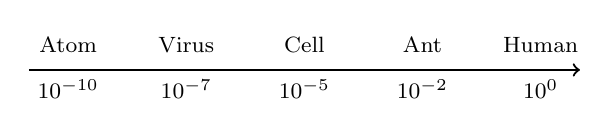
\begin{tikzpicture}[scale=0.5]
  \draw[thick,->] (0,0) -- (14,0);
  \node[below,font=\footnotesize] at (1,0) {$10^{-10}$};
  \node[below,font=\footnotesize] at (4,0) {$10^{-7}$};
  \node[below,font=\footnotesize] at (7,0) {$10^{-5}$};
  \node[below,font=\footnotesize] at (10,0) {$10^{-2}$};
  \node[below,font=\footnotesize] at (13,0) {$10^{0}$};
  \node[above,font=\footnotesize] at (1,0.2) {Atom};
  \node[above,font=\footnotesize] at (4,0.2) {Virus};
  \node[above,font=\footnotesize] at (7,0.2) {Cell};
  \node[above,font=\footnotesize] at (10,0.2) {Ant};
  \node[above,font=\footnotesize] at (13,0.2) {Human};
\end{tikzpicture}
\end{center}
\end{questionText}
\choiceA{Atom}
\choiceB{Virus}
\choiceC{Cell}
\choiceD{Ant}
\correctAnswer{C}
\explanation{$2 \times 10^{-5}$ is on the order of $10^{-5}$, which corresponds to a cell on the scale.}
\end{practiceQuestion}

\begin{practiceQuestion}{3-11-q25}{gsa}
\begin{questionText}
Complete the table by writing each number in scientific notation.

\begin{center}
\begin{tabular}{|c|c|}
\hline
\textbf{Standard Form} & \textbf{Scientific Notation} \\
\hline
$250{,}000$ & ? \\ \hline
$0.0034$ & ? \\ \hline
\end{tabular}
\end{center}
\end{questionText}
\correctAnswer{$250{,}000 = 2.5 \times 10^5$ and $0.0034 = 3.4 \times 10^{-3}$}
\explanation{$250{,}000$: move $5$ places left → $2.5 \times 10^5$. $0.0034$: move $3$ places right → $3.4 \times 10^{-3}$.}
\end{practiceQuestion}

\begin{practiceQuestion}{3-11-q26}{gsa}
\begin{questionText}
The bar graph compares masses of objects in scientific notation. About how many times heavier is Object B than Object A?

\begin{center}
\begin{tikzpicture}[scale=0.5]
  \draw[thick,->] (0,0) -- (0,6);
  \draw[thick,->] (0,0) -- (5,0);
  \node[left,font=\footnotesize,rotate=90] at (-0.8,3) {Mass (kg)};
  \node[left,font=\footnotesize] at (-0.2,2) {$10^2$};
  \node[left,font=\footnotesize] at (-0.2,5) {$10^5$};
  \fill[funBlue] (1,0) rectangle (2,2);
  \fill[funGreen] (3,0) rectangle (4,5);
  \node[below,font=\footnotesize] at (1.5,-0.2) {A};
  \node[below,font=\footnotesize] at (3.5,-0.2) {B};
\end{tikzpicture}
\end{center}
\end{questionText}
\correctAnswer{$1{,}000$ times heavier}
\explanation{$\dfrac{10^5}{10^2} = 10^3 = 1{,}000$. Object B is $1{,}000$ times heavier than Object A.}
\end{practiceQuestion}

\begin{practiceQuestion}{3-11-q27}{gsa}
\begin{questionText}
Order the following from least to greatest.

\begin{center}
\begin{tabular}{|c|}
\hline
$7.1 \times 10^{-2}$ \\ \hline
$3.5 \times 10^{1}$ \\ \hline
$9.9 \times 10^{-4}$ \\ \hline
$1.2 \times 10^{3}$ \\ \hline
\end{tabular}
\end{center}
\end{questionText}
\correctAnswer{$9.9 \times 10^{-4},\ 7.1 \times 10^{-2},\ 3.5 \times 10^{1},\ 1.2 \times 10^{3}$}
\explanation{Convert: $0.00099,\ 0.071,\ 35,\ 1{,}200$. Order from least to greatest by comparing exponents first, then coefficients.}
\end{practiceQuestion}
